\chapter{Resultados}
\label{chp:resultados}

\section{Introducción}

En el presente capítulo se presenta, de manera secuencial, los resultados de la exploración general llevada a cabo en laboratorio para buscar la evidencia de la formación del organogel en el sistema multifásico aceite-salmuera-surfactante (\textbf{A-S-S}). El trabajo realizado incluye la preparación de varias series de pruebas de botella, mediciones reométricas, y toma de imágenes de microscopía. La descripción técnica de los equipos de laboratorio utilizados se incluye el anexo A.

\section{Pruebas de botella}

Luego de la preparación del sistema \textbf{A-S-S} y el agitamiento dentro de las botellas, se forman al menos dos fases líquidas (agua libre y  emulsión o gel), y espuma, esta última puede romperse dependiendo del manejo de la botella. Las fases mencionadas se muestran en la \autoref{fig:botellas}.

\begin{figure}\centering
    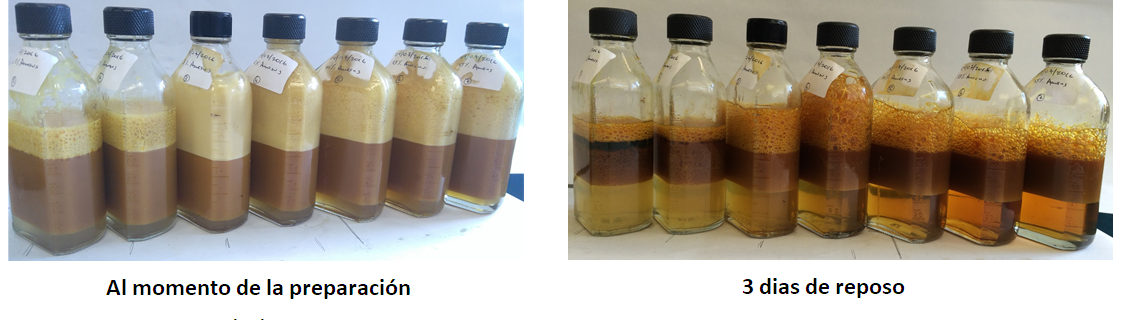
\includegraphics[width=1.0\textwidth]{Experimental/Botellas_2.png}
    \caption[Fases formadas en botellas]{Pruebas de botella realizadas para el sistema \textbf{A-S-S} a diferentes concentraciones de surfactante Amesus 3100}
    \label{fig:botellas}
\end{figure}

Mediante análisis de imágenes y con la ayuda de un simple algoritmo para contar los pixeles en cada imagen, se registraron los niveles aproximado en $mL$. La medición de los niveles de agua libre y la parte emulsionada (organogel) se presentan en la \autoref{fig:drene2}. 

\begin{figure}[H]\centering 
    \subfloat[Agua libre]{
        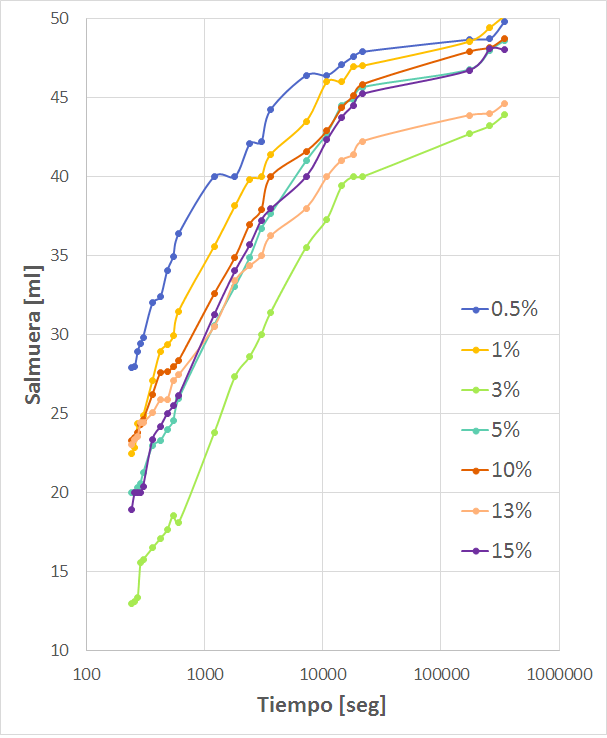
\includegraphics[width=0.5\textwidth]{Experimental/drene1.png} }
    \subfloat[Emulsión organogel]{
        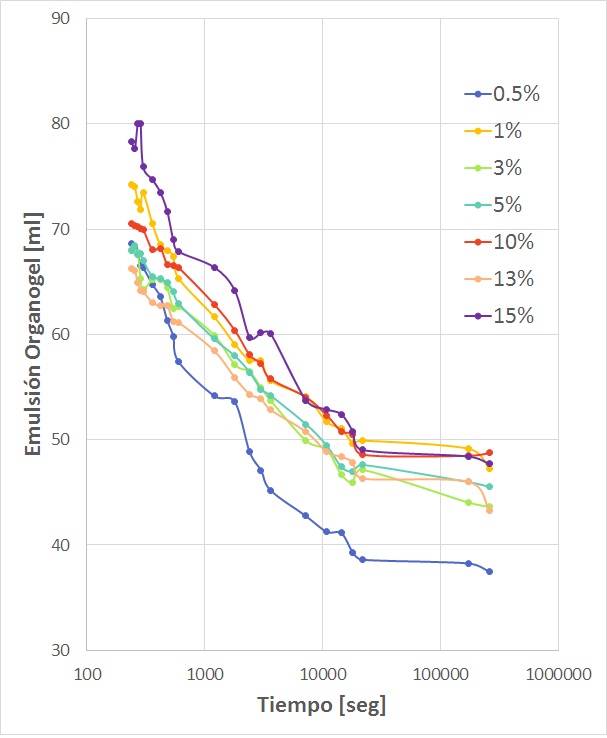
\includegraphics[width=0.5\textwidth]{Experimental/drene2.png} }
    \caption[Drenado de las fases]{Gráfico donde se muestran los niveles de ambas fases agua libre, y emulsión organogel durante $10$ días a $70 \celsius $ para $7$ concentraciones de producto surfactante Amesus $3100$ . }
    \label{fig:drene2}
\end{figure}

En este gráfico la dispersión de los puntos al final de drenado se ve afectada por la cantidad de espuma que sobrevivió en el horno y que se muestra en la figura anterior. Por ello se analizó la muestra de espuma al microscopio para comparar su morfología con la de la parte emulsión gel. Esta comparación se muestra en la \autoref{fig:comparativa}.

\begin{figure}[H]\centering 
    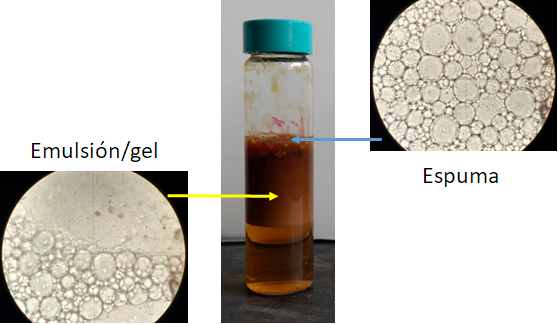
\includegraphics[width=0.8\textwidth]{Experimental/comparativa.png}
    \caption[Morfología de espuma]{Se realizó una prueba de botella para comparar la morfología de la espuma formada después del agitamiento en los casos en las concentraciones para las que sobrevivió la espuma después del calentamiento. }
    \label{fig:comparativa}
\end{figure}

No se encontraron diferencias en la morfología de la espuma respecto a la del gel, por lo que se presume que su composición es básicamente la misma, con la única diferencia siendo aire atrapado por la una película de surfactante.

\section{Reometría}
Para cada fase presente en las pruebas de botella, se realizaron las pruebas descritas en el capítulo anterior. Se encontraron los siguientes reogramas:

\subsection{Emulsión organogel}

    \subsubsection{Prueba A}
    La viscosidad del sistema se ve afectado por la concentración de surfactante, al momento de la preparación, un incremento de concentración viene acompañado de una viscosidad mayor, la cual en todos los casos se incrementa después de 24 hrs. Sin embargo la relación antes mencionada entre viscosidad y concentración no prevalece pasadas las 24 hrs.(\autoref{fig:AR06}).
    
    \begin{figure}[h]
        \centering
        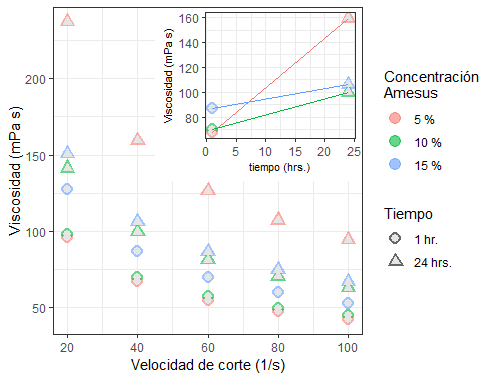
\includegraphics[width=0.9\textwidth]{R_plot/Rplot06.png}
        \caption[Prueba A emulsión organogel]{Emulsión-organogel Prueba A: $14.7$ [psi] y $23~\celsius$.}
        \label{fig:AR06}
    \end{figure}
    
    \subsubsection{Prueba B}
    En esta prueba, la presión del sistema se refleja en una menor viscosidad en todos los casos. El incremento de viscosidad con la concentración también se cumple al momento de la preparación. Esta relación no se cumple pasadas las 24 hrs. (\autoref{fig:BR07}).
    
    \begin{figure}[h]
        \centering
        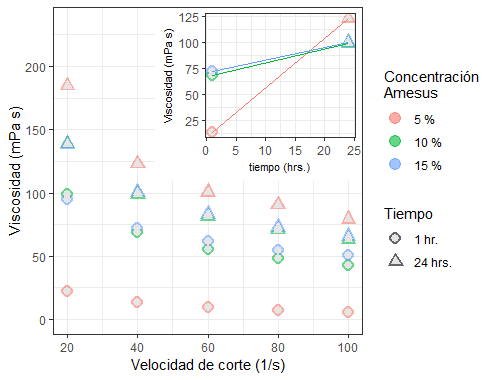
\includegraphics[width=0.9\textwidth]{R_plot/Rplot07.png}
        \caption[Prueba B emulsión organogel]{Emulsión-organogel Prueba B: $1500$ [psi] y $23~\celsius$.}
        \label{fig:BR07}
    \end{figure}

    \subsubsection{Prueba C}
    La temperatura del sistema reduce la viscosidad de la muestra en todos los casos, se presume que también la presión contribuye a este comportamiento. Al momento de la preparación una mayor concentración de surfactante incrementa la viscosidad, sin embargo pasadas 24 hrs. esta tendencia se invierte teniendo viscosidades mas bajas para concentraciones mas altas de producto. (\autoref{fig:CR08}).
    
    \begin{figure}[h]
        \centering
        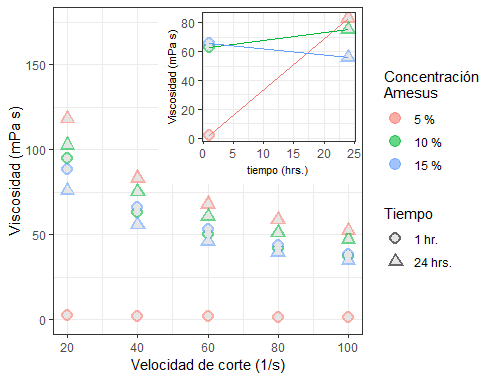
\includegraphics[width=0.9\textwidth]{R_plot/Rplot08.png}
        \caption[Prueba C emulsión organogel]{Emulsión-organogel Prueba C: $1500$ [psi] y $160~\celsius$.}
        \label{fig:CR08}
    \end{figure}

    \subsubsection{Prueba D}
    El incremento constante de la temperatura del sistema tiene como resultado la disminución de la viscosidad de la muestra en todos los casos. La concentración muestra un efecto similar que la prueba \textbf{C}. Alrededor de los $100 \celsius$ esta tendencia se invierte aumentando la viscosidad de la muestra con la temperatura, lo que podría ser indicio de la aparición de estructuras. (\autoref{fig:DR09}).
    
    \begin{figure}[h]
        \centering
        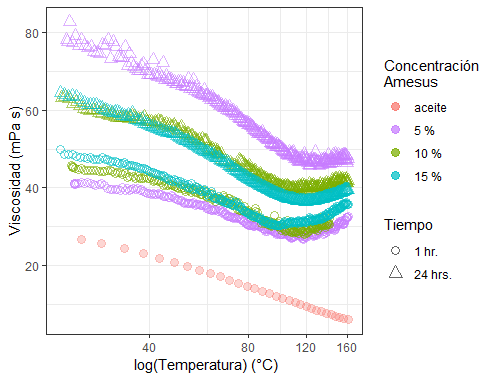
\includegraphics[width=0.9\textwidth]{R_plot/Rplot09.png}
        \caption[Prueba D emulsión organogel]{Emulsión-organogel Prueba D: $100~[s^{-1}]$ y $23~-~160~\celsius$.}
        \label{fig:DR09}
    \end{figure}


\subsection{Salmuera}

    \subsubsection{Prueba A}
     El aumento de la concentración de surfactante disponible en el sistema incrementa la viscosidad del sistema, el tiempo después de la preparación influye de manera significativa para al concentración mas alta, mientas que en las demás no es tan importante \autoref{fig:AR10}.
    
    \begin{figure}[h]
        \centering
        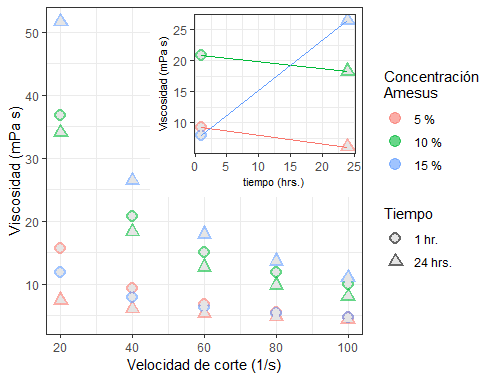
\includegraphics[width=0.9\textwidth]{R_plot/Rplot10.png}
        \caption[Prueba A salmuera]{Salmuera Prueba A: $14.7$ [psi] y $23~\celsius$.}
        \label{fig:AR10}
    \end{figure}
    
    \subsubsection{Prueba B}
    La presión del sistema reduce la viscosidad de las muestras en todos los casos respecto a la prueba anterior \autoref{fig:BR11}.
    
    \begin{figure}[h]
        \centering
        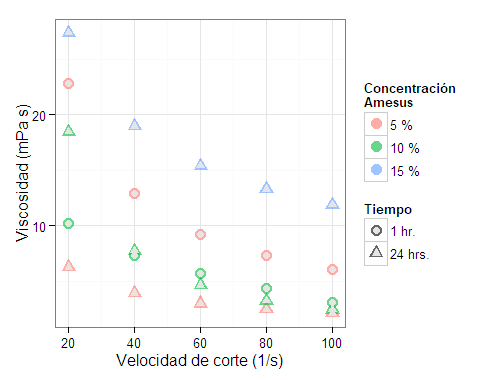
\includegraphics[width=0.9\textwidth]{R_plot/Rplot11.png}
        \caption[Prueba B salmuera]{Salmuera Prueba B: $1500$ [psi] y $23~\celsius$.}
        \label{fig:BR11}
    \end{figure}
    
    \subsubsection{Prueba C} 
    No pudo realizarse dado que la resolución del equipo no lo permite.
    
    \subsubsection{Prueba D}
    descripción. \autoref{fig:DR12}
    
    \begin{figure}[h]
        \centering
        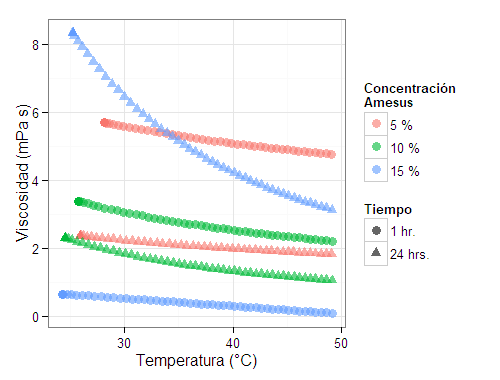
\includegraphics[width=0.9\textwidth]{R_plot/Rplot12.png}
        \caption[Prueba D salmuera]{Salmuera Prueba D: $100~[s^{-1}]$ y $23~-~50~\celsius$. La prueba no alcanza la temperatura final programada, pues la viscosidad del sistema está en el umbral de detección del reómetro, por lo que se decide detenerla a $50\celsius$.}
    \label{fig:DR12}
\end{figure}


\subsection{Aceite libre}
    \subsubsection{Prueba D}
    El aumento en la concentración de surfactante incrementa la viscosidad de la muestra, mientras que la temperatura tiene el efecto contrario. A pesar de esto en todos los casos la viscosidad del aceite sin el producto es mucho mayor 
    \begin{figure}[h]
        \centering
        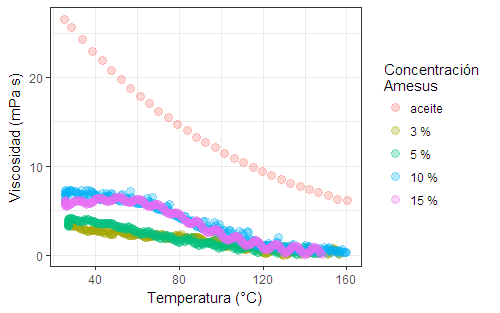
\includegraphics[width=0.9\textwidth]{R_plot/Rplot13.png}
        \caption[Prueba D aceite]{Aceite libre Prueba D: $100~[s^{-1}]$ y $23~-~160~\celsius$.}
        \label{fig:Daceite}
    \end{figure}


\subsection{Efecto de la salinidad}

%\begin{description}
%    \item[Prueba A] descripción. \autoref{fig:Asalmu}
%    \item[Prueba B] descripción. \autoref{fig:Bsalmu}
%    \item[Prueba D] descripción. \autoref{fig:Dsalmu}
%\end{description}
%
%\begin{figure}[h]
%    \centering
%    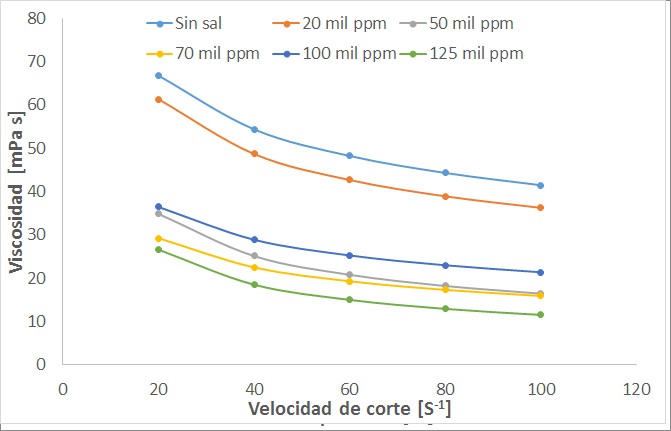
\includegraphics[width=\textwidth]{Experimental/A_sali.png}
%    \caption[Prueba A salinidad]{Salinidad Prueba A: $14.7$ [psi] y $23~\celsius$.}
%    \label{fig:Asal}
%\end{figure}
%
%\begin{figure}[h]
%    \centering
%    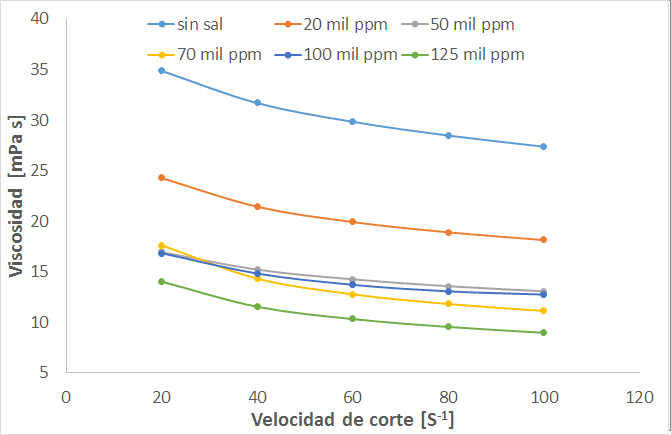
\includegraphics[width=\textwidth]{Experimental/B_sali.png}
%    \caption[Prueba B salinidad]{Salinidad Prueba B: $1500$ [psi] y $23~\celsius$.}
%    \label{fig:Bsal}
%\end{figure}
%
%\begin{figure}[h]
%    \centering
%    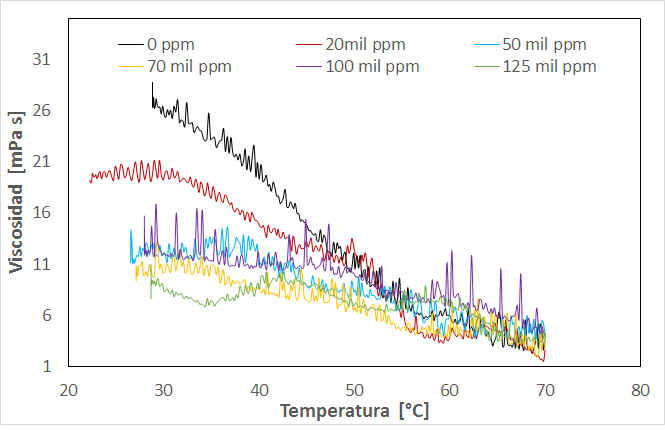
\includegraphics[width=\textwidth]{Experimental/D_sali.png}
%    \caption[Prueba D salinidad]{Salinidad Prueba D: $100~[s^{-1}]$ y $23~-~160~\celsius$.}
%    \label{fig:Dsal}
%\end{figure}
%
%\begin{figure}[h]
%    \centering
%    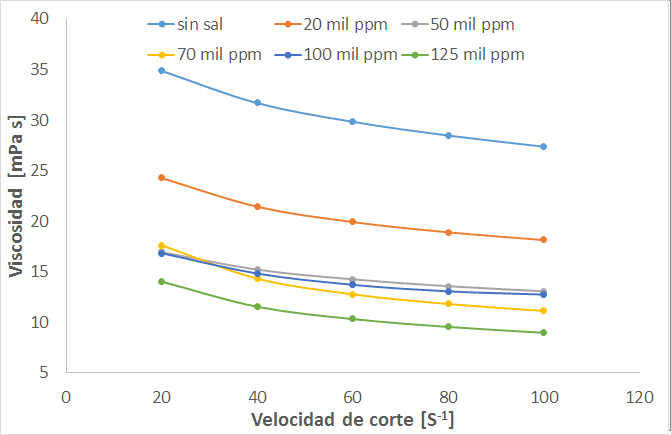
\includegraphics[width=\textwidth]{Experimental/F_sali.png}
%    \caption[Prueba F salinidad]{Salinidad Prueba F: $1500$ [psi] y $70~\celsius$.}
%    \label{fig:Fsal}
%\end{figure}

Se confirma a través de las pruebas \textbf{A B D F} que la salinidad afecta el desempeño del agente surfactante. En la mayoría de los pruebas se puede observar que la concentración intermedia del sistema ($10\%$) representa un estado de transición que se refleja en sus propiedades. Lo anterior indica que para establecer una relación entre salinidad y viscosidad se requiere un estudio más amplio que está fuera de los alcances de este trabajo.


\subsection{Esfuerzo de cedencia}

Para las serie de muestras preparada, se identificaron nuevamente dos fases, agua libre y organogel respectivamente las pruebas $G1$ y $G2$ produjo los reogramas presentados en la \autoref{fig:cedencia1} y \autoref{fig:cedencia2}, en donde se observa que todas las concentraciones y temperaturas presentan un cruce de las curvas de módulo complejo y módulo de almacenamiento, lo que confirma que se trata de una sustancia viscoelástica que posee un punto de cedencia. Aunque no se encontró una relación clara del punto de cedencia con respecto a la concentración esto puede deberse a la dificultad para el muestreo pues la interfase entre las zonas acuosa y oleosa se elige de manera arbitraria.

\begin{figure}[h]
    \centering
    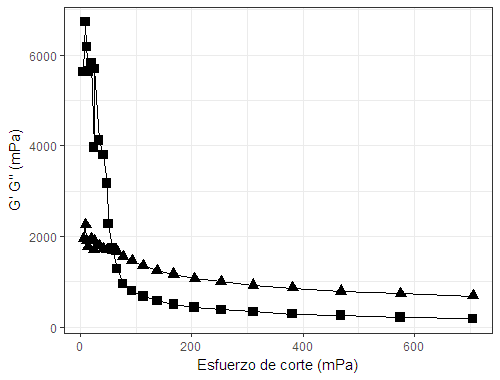
\includegraphics[width=0.9\textwidth]{R_plot/Rplot14.png}
    \caption[Punto de cedencia]{Punto de cedencia, reograma típico de la prueba G1. Las curvas del reograma representan el módulo de pérdida y el de almacenamiento, los cuales se cruzan justo en el el punto de cedencia.}
    \label{fig:cedencia1}
\end{figure}

\begin{figure}[h]
    \centering
    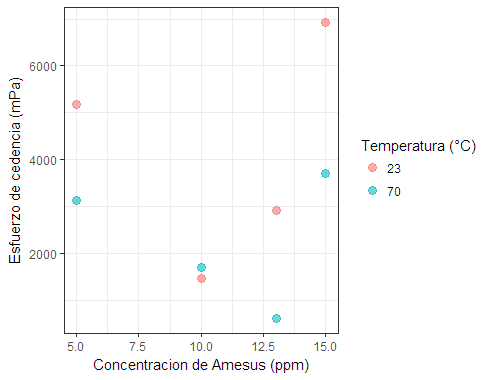
\includegraphics[width=0.9\textwidth]{R_plot/Rplot15.png}
    \caption[Prueba G$2$ ]{Punto de cedencia vs concentración de surfactante, resumen de las pruebas G$1$ y G$2$: $\omega = 0.5~rad/s$.}
    \label{fig:cedencia2}
\end{figure}


Los valores de punto de cedencia vs concentración de cada una de las fases emulsionadas (clara y oscura) se encuentran resumidos en la \autoref{tab:cedencia}. En todos los casos el esfuerzo de cedencia disminuye con la temperatura. De manera general se aprecia que independiente de la frecuencia angular el punto de cedencia es similar, este comportamiento corresponde con la clasificación propuesta para un gel débil o fluido estructurado (\cite{Clark}).

  \begin{table}
    \caption[Punto de cedencia]{\raggedright Esfuerzo de cedencia a diferentes concentraciones de producto y temperatura.}
    \centering \settowidth\tymin{\textbf{Teotleco}} \setlength\extrarowheight{2pt} \footnotesize
    \begin{tabulary}{1.1\textwidth }{|L|L|L L L L L L|}
        \toprule 
        Gota & Densidad &  \multicolumn{6}{c|}{IFT [$dyn/cm^{2}$]} \\
        \midrule
        Teotleco & $0.824423$ & $19.45$ & $10.88$ & $8.23$ & $6.11$ & $3.64$ & $1.64$ \\
        \cmidrule{1-2} %\midrule[20pt]
        \multicolumn{2}{|l|}{Concentración [ppm]} & $1$ & $56.25$ & $290$ & $625$ & $1250$ & $2500$ \\
        %\midrule
        \multicolumn{2}{|l|}{Densidad del medio } & $1.1614$ & $1.16135$ & $1.16109$ & $1.16064$ & $1.15936$ & $1.15765$\\
        \midrule
        \bottomrule
    \end{tabulary}
    \label{tab:cedencia}
\end{table}

\section{Análisis de Imágenes}

\begin{figure}[h]
    \centering
    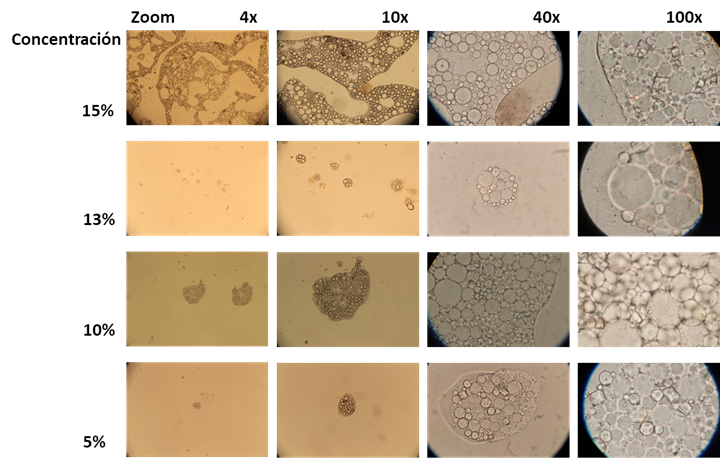
\includegraphics[width=\textwidth]{Experimental/Amesus_Botellas.png}
    \caption[Microscopia Amesus 3100 ]{Microscopía de la muestra de Amesus $3100$. En orden descendente, botellas $4$ a la $7$.}
    \label{fig:micro1}
\end{figure}

% \begin{figure}[h]
%     \centering
%     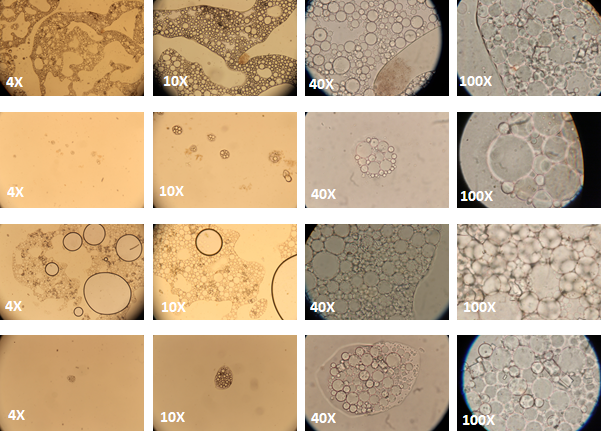
\includegraphics[width=\textwidth]{Experimental/Amesus_3200_Botellas.png}
%     \caption[Microscopia Amesus 3200 ]{Microscopía de la muestra de Amesus $3200$. En orden descendente, botellas $4$ a la $7$.}
%     \label{fig:micro2}
% \end{figure}


\section{Tensión interfacial}

El sistema \textbf{Aceite-S-S}, se midió en todo el rango de concentraciones con éxito sin embargo los intentos por medir el sistema Organogel-S-S no tuvieron la misma consistencia dado que el organogel no forma gotas en la punta del capilar, el detalle de este fenómeno se puede observar en la \autoref{fig:IFT_pic}

\begin{figure}\centering
    \subfloat[]{
    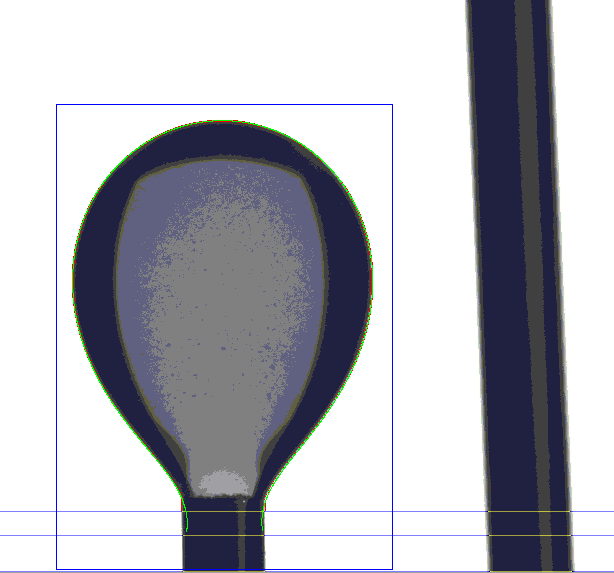
\includegraphics[width=0.44\textwidth]{Experimental/IFT_pic.png}} \quad
    \subfloat[]{
    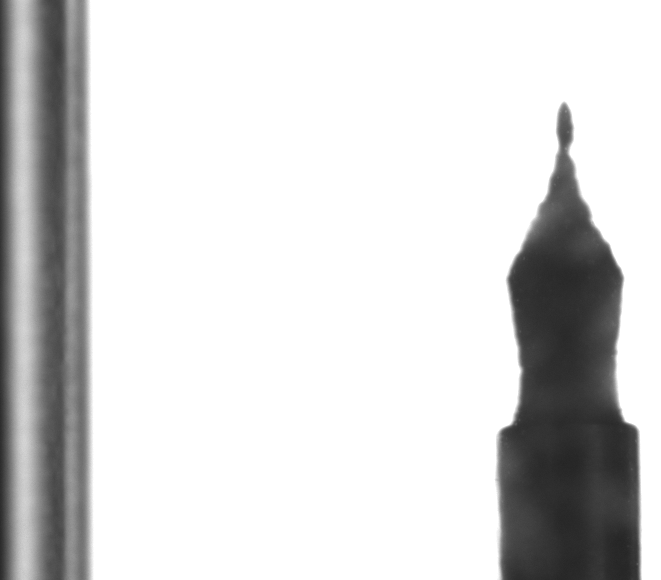
\includegraphics[width=0.44\textwidth]{Experimental/IFT_pic2.png}}
    \caption[Fotorgrafías gotas]{\textbf{(a)} Sistema Aceite-Salmuera-Surfactante, el aceite forma gotas que flotan debido a la diferencia de densidad. \textbf{(b)} Sistema Organogel-Salmuera-Surfactante, en ninguna concentración el gel forma gotas.}
    \label{fig:IFT_pic}
\end{figure}


Los valores de tensión interfacial para, el sistema \textbf{Aire-S-S} y para \textbf{Aceite-S-S} a diferentes concentraciones de surfactante se encuentran resumidos en la \autoref{tab:IFTtab1} y la \autoref{tab:IFTtab2}

  \begin{table}
    \caption[Tensión interfacial sistema Aire-Salmuera]{\raggedright Tensión interfacial sistema Aire-Salmuera vs concentración de surfactante Amesus $3200$.}
    \centering \settowidth\tymin{\textbf{Teotleco}} \setlength\extrarowheight{2pt} \footnotesize
    \begin{tabulary}{1.1\textwidth }{|L|C|L L L L L L|}
        \toprule 
        Tipo & Fase &  \multicolumn{6}{c|}{Densidad [$g/cm^{3}$]} \\
        \midrule
        Gota & líquido & $19.45$ & $10.88$ & $8.23$ & $6.11$ & $3.64$ & $1.64$ \\
        Medio & gas & $1.0014$ & $0.00135$ & $1.00109$ & $1.00064$ & $1.00936$ & $0.00765$\\
        \midrule
        \multicolumn{2}{|l|}{Concentración [ppm]} & $1$ & $56.25$ & $290$ & $625$ & $1250$ & $2500$ \\
\multicolumn{2}{|l|}{IFT ~~~~~~~~~[$dyn/cm^{2}$]} & $66.664$ & $58.0$ & $290$ & $625$ & $1250$ & $2500$ \\
        \midrule
        \bottomrule
    \end{tabulary}
    \label{tab:IFTtab1}
\end{table}

  \begin{table}
    \caption[Tensión interfacial sistema Aceite-Salmuera]{\raggedright Tensión interfacial sistema Aceite-Salmuera vs concentración de surfactante Amesus $3200$.}
    \centering \settowidth\tymin{\textbf{Teotleco}} \setlength\extrarowheight{2pt} \footnotesize
    \begin{tabulary}{1.1\textwidth }{|L|L|L L L L L L|}
        \toprule 
        Gota & Densidad &  \multicolumn{6}{c|}{IFT [$dyn/cm^{2}$]} \\
        \midrule
        Teotleco & $0.824423$ & $19.45$ & $10.88$ & $8.23$ & $6.11$ & $3.64$ & $1.64$ \\
        \cmidrule{1-2} %\midrule[20pt]
        \multicolumn{2}{|l|}{Concentración [ppm]} & $1$ & $56.25$ & $290$ & $625$ & $1250$ & $2500$ \\
        %\midrule
        \multicolumn{2}{|l|}{Densidad del medio } & $1.1614$ & $1.16135$ & $1.16109$ & $1.16064$ & $1.15936$ & $1.15765$\\
        \midrule
        \bottomrule
    \end{tabulary}
    \label{tab:IFTtab2}
\end{table}


\begin{figure}
    \centering
    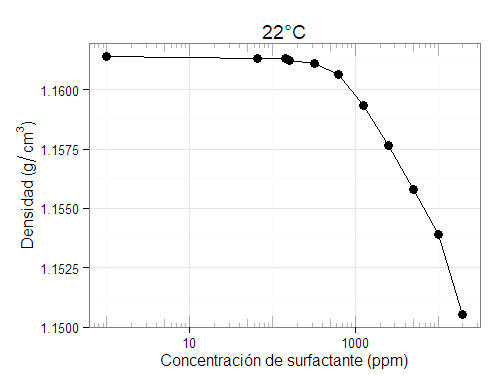
\includegraphics[width=0.9\textwidth]{R_plot/Rplot23.png}
    \caption[Densidad del sistema Aire-S-S.]{Densidad del sistema Aire-Salmuera-Surfactante \emph{Vs} concentración de surfactante.}
    \label{fig:denAireSS}
\end{figure}

\begin{figure}
    \centering
    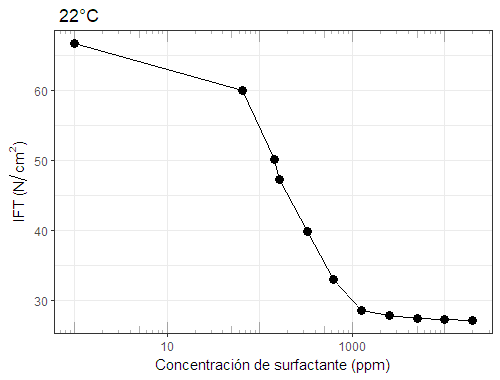
\includegraphics[width=0.9\textwidth]{R_plot/Rplot24.png}
    \caption[IFT del sistema Aire-S-S.]{Tensión interfacial del sistema Aire-Salmuera-Surfactante \emph{Vs} concentración de surfactante.}
    \label{fig:IFTAireSS}
\end{figure}



\begin{figure}
    \centering
    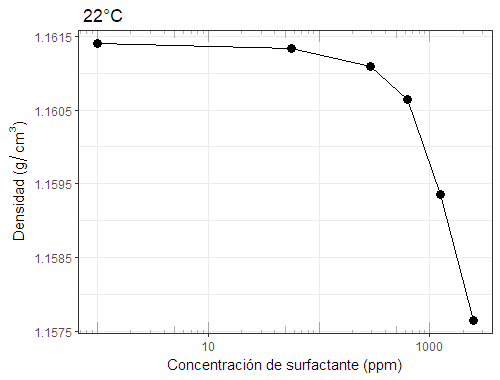
\includegraphics[width=0.9\textwidth]{R_plot/Rplot25.png}
    \caption[Densidad del sistema A-S-S.]{Densidad del sistema Aceite-Salmuera-Surfactante vs concentración de surfactante.}
    \label{fig:denASS}
\end{figure}

\begin{figure}
    \centering
    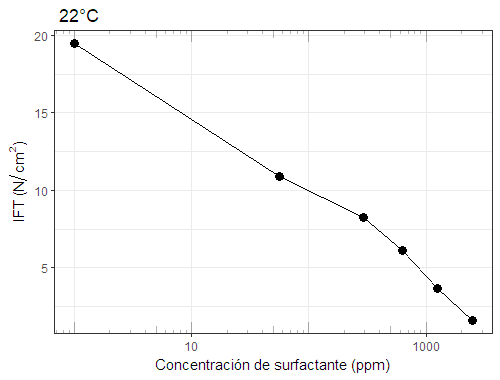
\includegraphics[width=0.9\textwidth]{R_plot/Rplot26.png}
    \caption[IFT del sistema A-S-S.]{Tensión interfacial del sistema Aceite-Salmuera-Surfactante \emph{Vs} concentración de surfactante.}
    \label{fig:IFTASS}
\end{figure}
